El control de cortinas es un proceso que combina elementos mecánicos
y eléctricos con el fin de \textbf{controlar la posición de la cortina} de manera
manual o automática, ajustando la posición mediante el control del voltaje
aplicado al motor (ajustando la cantidad de pulsos).

\subsubsection{Principio de funcionamiento}

El sistema consiste de una cortina de lino enrollable de $\SI{1,4}{\meter}$ de ancho y $\SI{1,2}{\meter}$ de alto con una base de madera que hace contrapeso, se enrolla alrededor de un eje de $\SI{1,5}{\centi\meter}$ de radio.
Además cuenta con un motor de corriente continua controlado por tensión \textbf{Faulhaber 2250-BX4} cuyo eje de salida está conectado a una caja reductora \textbf{Faulhaber 26A} con relación de transmisión 40 a 1 y éste a su vez al eje de la cortina, del otro lado el motor, tiene conectado un sensor rotativo incremental \textbf{Faulhaber IE3-1024} el cual envía datos de posición relativa mediante señales digitales eléctricas operando en 1024 pulsos por revolución, y una placa de desarrollo \textbf{Arduino Uno R3}, este recibe las señales digitales del sensor rotativo, interpreta la posición de la cortina y genera señales PWM. La señal PWM generada por el Arduino excita directamente a un driver de potencia puente H \textbf{IBT-2} que controla la tensión que recibe el motor.

\begin{figure}[h]
	\centering
	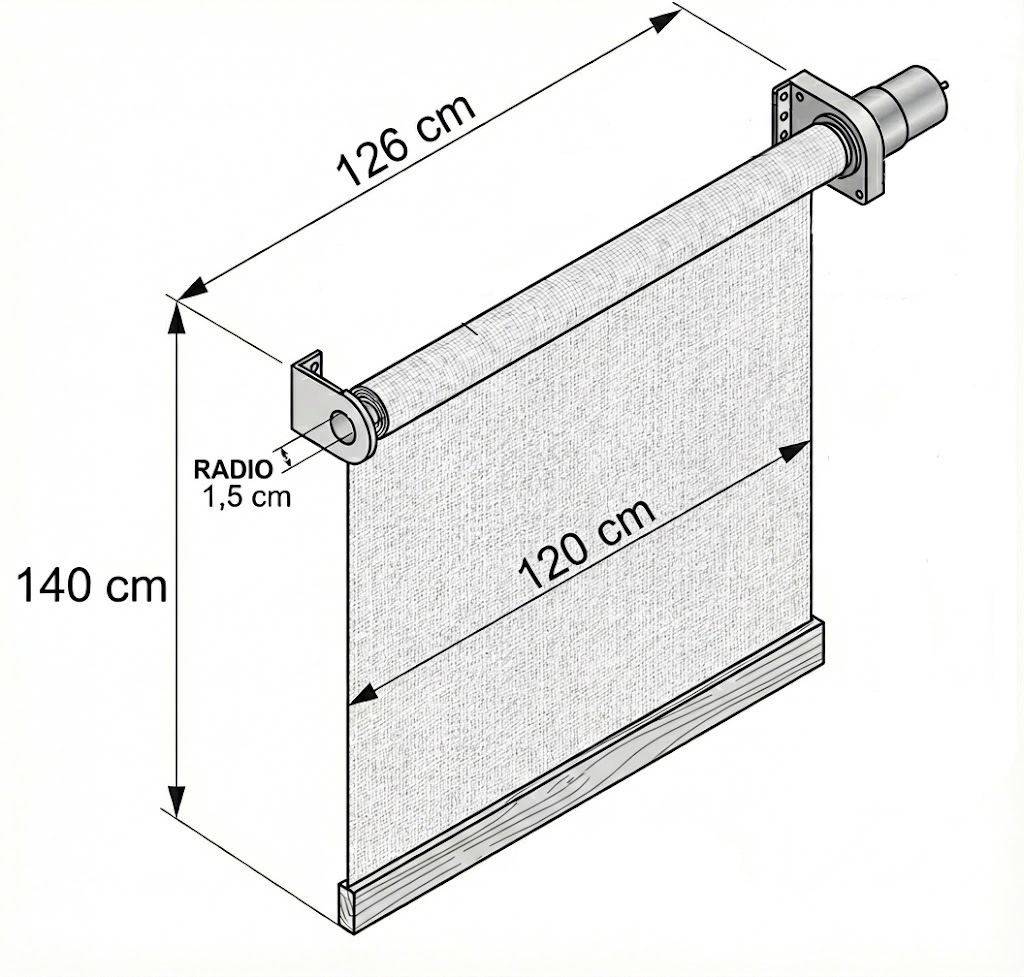
\includegraphics[width=0.65\textwidth]{img/esquema_fisico_sistema.png}
	\caption{Esquema físico del sistema.}
	\label{fig:esquema fisico}
\end{figure}
\subsubsection{Posibles perturbaciones}
\label{pos_pert}
Las perturbaciones que afectan el desempeño del sistema se manifiestan principalmente como variaciones en la carga mecánica inherentes al mecanismo de enrollado entre otros factores. Las perturbaciones más significativas son:
\begin{itemize}
	\item El par gravitatorio constante generado por el peso de la cortina y el contrapeso, los cuales introduce una asimetría operativa, exigiendo mayor torque para vencer la gravedad durante el ascenso que durante el descenso.
	\item La variación del radio efectivo del eje, el cual aumenta progresivamente al enrollarse la tela, incrementando el brazo de palanca y la demanda de par a medida que la cortina gana altura.
	\item Fluctuaciones en la tensión de la fuente de alimentación que impactan directamente en la respuesta dinámica del motor.
\end{itemize}

\subsubsection{No linealidades}
\label{no_linealidades}

Las no linealidades más significativas del sistema son:

\begin{itemize}
	\item Saturación: Limitación de la tensión aplicada al motor a un rango finito, representando las restricciones físicas de la fuente de alimentación y de la etapa de potencia. Esta no linealidad impide que la acción de control crezca indefinidamente ante errores grandes.
	
	\item Zona muerta: Modela la existencia de un umbral mínimo de tensión por debajo del cual el motor no produce movimiento, principalmente debido a la fricción estática del conjunto mecánico y de la caja reductora, lo que dificulta la corrección de errores pequeños.
	
	\item Cuantización: Derivada de la naturaleza discreta del sensor rotativo (encoder). Al transformar el desplazamiento angular continuo en una serie de pulsos digitales, se introduce un error de redondeo intrínseco. Aunque su magnitud es pequeña, puede provocar oscilaciones de baja amplitud alrededor del punto de referencia, ya que el controlador no puede resolver errores menores al tamaño de un pulso.

\end{itemize}